%%%%%%%%%%%%%%%%%%%%%%%%%%%%%%%%%%%%%%%%%%%%%%%%%%%%%%%%%%%%%%%%%%%%%%%%%%%%%%%%%%%%%%%%%%%%%%%%%%%%%%%
% Soutenance 1
% Bitume Legends Project
% CarrEniX
% Mars 2022
%%%%%%%%%%%%%%%%%%%%%%%%%%%%%%%%%%%%%%%%%%%%%%%%%%%%%%%%%%%%%%%%%%%%%%%%%%%%%%%%%%%%%%%%%%%%%%%%%%%%%%%

% Packages
\documentclass[12pt,a4paper]{article}
\usepackage{mathtools}
\usepackage[utf8]{inputenc}
\usepackage{graphicx}
\usepackage[french]{babel}
\usepackage[T1]{fontenc}
\usepackage{url}
\usepackage{fancyhdr}
\usepackage{longtable}
\usepackage[aboveskip=.5cm]{caption}
\usepackage{pdflscape}
\usepackage{geometry}

% Global settings of document
\setlength\parindent{20pt}
\newcommand{\btmlgs}{\textsl{Bitume Legends}}
\newcommand{\AI}{Intelligence Artificielle}
\newcommand{\CEX}{\textsc{CarrEniX}}
\pagestyle{fancy}
\rhead{\btmlgs}
\lhead{Rapport de Première Soutenance}
\rfoot{Page \thepage}
\lfoot{\CEX}
\fancyfoot[C]{}
\setlength{\headheight}{15pt}
\geometry{textheight=600pt}
\renewcommand{\listfigurename}{Table des Annexes}
\renewcommand{\contentsname}{Table des Matières}
\graphicspath{{../Medias}}

% Begin of the document
\begin{document}

\begin{titlepage}
  \newcommand{\HRule}{\rule{\linewidth}{0.5mm}}
  \center
  \text{\LARGE Projet \btmlgs}\\[1cm]
   
\includegraphics[scale=0.7]{logo192.png} \\[1cm]
    \HRule \\[0.4cm]
    { \huge \bfseries Rapport de Première Soutenance\\[0.3cm] }
    \HRule \\[1.5cm]
    {\large \bfseries \CEX} \\[0.3cm]
    Anthony \textsc{Caron}\;--\;Melvyn \textsc{Delaroque}\\
    Victorien \textsc{Cambourian}\;--\;Xavier \textsc{de Place}
    \\ [6cm]
    EPITA INFOSUP 2026\\Année 2021 - 2022\\
    \(\mathtt{btms.games}\)
\end{titlepage}

\tableofcontents
\clearpage

\addcontentsline{toc}{section}{Introduction}
\section*{Introduction}
    Nous sommes le studio \CEX\, qui développe \btmlgs, un jeu de course automobile 3D réaliste en
    \textit{low-poly}. Après avoir commencé le projet début janvier, nous publions notre 
    premier rapport. Il permet de faire le point sur ce que nous avons fait, les objectifs
    atteints, les priorités ainsi que les ressources utilisés durant ce projet. Dans ce rapport,
    nous allons aborder l'avancée de notre projet, l'organisation de notre groupe, les 
    ressources et créations de chacun des membres du groupe ainsi que leurs valeurs 
    ajoutées, le ressenti des membres durant cette première période et nos objectifs.
  
\section{Avancée du Projet}
    \subsection{Multijoueur}
        La base du multijoueur a été implémentée, non sans peines. 
        Nous pouvons nous connecter à 4 personnes (nous avons choisi ce nombre pour des questions 
        de simplicité) et commencer une partie. Il y a une interface de connection, avec différentes 
        options (détaillées plus tard dans ce document) puis le système de \textit{spawn} (apparition).
        Une musique de jeu a également été crée pour le multijoueur.
  
    \subsection{Programme Beta (\(\beta\))}
        Nous avons créé un questionnaire sur \textsl{Google Forms} afin que les premières personnes testant
        le jeu puisse nous signaler les bugs qu'ils ont rencontrés et nous les décrire le plus 
        précisément possible dans le but d'être corrigé rapidement. Pour cela, ce questionnaire 
        possède pour trois catégories. Tout d'abord, une question sur le mode de jeu où le bug 
        s'est produit. Puis une autre sur la nature du bug et enfin un paragraphe réservé
        pour nous décrire avec le plus de détails possible ce bug. Toutefois, si l'utilisateur
        trouve compliqué de décrire son bug, des liens pour nous contacter sur \textsl{Discord} 
        ou \textsl{GitHub} sont indiqués.
  
    \subsection{Communication}
        Au sujet de la communication, nous avons décidé de faire une publication sur \textsl{Instagram}
        \footnote{\(\mathtt{instagram.com/bitumelegends}\)}
        pour tenir informés nos potentiels premiers joueurs. Dans cette publication se trouve le lien 
        du site Internet où l'utilisateur pourra consulter se familiariser avec le menu de notre
        jeu, puisque le site reprend l'esthétique de ce dernier. Enfin l'onglet de la réalisation
        et celui de la présentation donnent l'occasion de nous connaître plus, de même pour le projet.
        Ils pourront enfin nous rejoindre sur \textsl{Discord} pour que nous puissions les inscrire dans le
        programme de tests.
  
    \subsection{Site Internet}
        Le site web a pour but de présenter les membres du groupe, leur rôle et leur avis sur le projet.
        Il présente aussi l'historique avec les idées de conception du jeu, du nom du jeu et celui du studio
        de développement. Ensuite, il nous permet d'expliquer comment nous avons réalisé le projet avec la
        chronologie de réalisation, c'est-à-dire les différentes étapes de réalisation du projet mais aussi
        les problèmes rencontrés et les solutions envisagées. Enfin, il contient aussi
        un espace dédié pour télécharger le projet et le jeu. Ce site est notre vitrine, il nous permet de faire
        la promotion de \btmlgs.
  
  
  
    \subsection{Menu}
        Le menu doit permettre d'accéder aux différents modes de jeux et fonctionnalités du jeu.
        Il doit servir de hub pour accéder au mode multijoueur, contre la montre et contre l'\AI.
        Il doit également permettre d'accéder au garage contenant les voitures du joueur. Un affichage
        du niveau du joueur, un bouton pour accéder à la remontée de bug et un menu d'options 
        sont également dans le menu du jeu. Au début du projet, le menu était basique. Il servait 
        simplement à pouvoir accéder aux différentes modes de jeux. Suite à cela, Melvyn et Victorien 
        ont commencé à travailler sur un design plus poussé que celui de base de \textsl{Unity}, 
        en adoptant notamment un thème de couleurs basé sur le logo du jeu. Tout d'abord, une
        ébauche du design a été réalisée sur Canva, dans le but de partager des idées sur le look
        final du menu. Ensuite nous avons implémenté le design dans le jeu, en insérant un fond
        et des espaces pour les futures fonctionnalités, en implémentant les boutons et en changeant
        leur design. Nous avons également implémenté le code couleur du design. Enfin, nous avons 
        ajouté des effets sonores et de couleurs aux boutons lorsqu'ils sont cliques ou lorsque
        la souris passe dessus. Une musique tourne également en fond dans le menu.

\clearpage

\section{Organisation interne chez \CEX}
    \subsection{Organisation Pratique}
        Nous avons mis en place une organisation particulière entre nous,
        car au début nous ne savions pas spécialement par où commencer.
        Chaque semaine, nous nous sommes réunis pour définir des 
        objectifs pour chacun, à faire durant la semaine suivante. Cela nous 
        a permis d’avoir des buts concrets sur le court terme et d'avancer plus 
        efficacement.

    \subsection{Répartition des Tâches}
        Nous nous sommes basés sur ce que nous avions annoncé dans notre Cahier des Charges :
        Melvyn s'est occupé des musiques d'ambiance, du \textit{Sound Design} de 
        notre jeu et du menu principal. Victorien a créé le premier circuit du jeu,
        il a implémenté le menu principal et a modélisé sur \textsl{Blender} une Formule 1.
        Anthony a géré le site Internet, les réseaux sociaux et le programme \(\beta\).
        Enfin, Xavier a implémenté le mode multijoueur, et le cœur du moteur de jeu,
        à savoir le système de direction des voitures.

    \subsubsection{Anthony}
        Pour le site Web, nous avons décidé de reprendre l'esthétique du
        menu de notre jeu vidéo. Pour cela, nous avons divisé le site web 
        en quatre parties, accessibles par quatre boutons amenant aux quatre 
        sous-pages de notre site. La première est la présentation du projet, dans laquelle
        nous avons écrit une courte introduction, l'historique et les membres
        de l'équipe. La seconde concerne la réalisation du projet, qui contient
        la chronologie de la réalisation, les problèmes rencontrés et solutions
        envisagées pour contrer ceux-ci. Ensuite, une troisième page nous 
        offre des liens de téléchargement du jeu pour Windows et macOS, et
        le projet en version complète ou allégée.
        Enfin, la dernière page permet l'accès aux différentes ressources
        (liens des images, sons, logiciels...). C'est une sorte de bibliothèque 
        des sources de notre projet.
        Ainsi, il me manquera plus qu'à faire fonctionner certains boutons et 
        liens et rendre le site responsive, c'est a dire un site qui s'adapte en 
        fonction de l'appareil depuis lequel on le consulte, et 
        régler quelques bugs d'affichages pour finaliser le site Web. 
    
\clearpage

    \subsubsection{Melvyn}
        Étant responsable de la musique, j'ai composé la 
        musique du jeu. J'ai utilisé le logiciel de MAO (Musique Assistée par Ordinateur) 
        \textsl{FL Studio 20}. J'ai composé deux musiques, une musique pour le menu et 
        une musique de course et j'ai demandé à un ami d'enregistrer sa voix pour la musique
        dans un studio d'enregistrement de son école. Le style choisi par mes pairs et moi-même
        au sein du groupe est la \textsl{Phonk}, style est souvent associé à la culture automobile
        \textit{underground} japonaise, d'où le désir d'utiliser de la \textsl{Phonk} pour notre jeu. 
        De plus, ce style est très énergique, assourdissant parfois et fait monter l'adrénaline
        dans le sang. Au début, j'ai hésité à faire de l'\textit{Eurobeat}, un genre de \textit{dance music}
        associé au milieu automobile, mais le groupe a tranché et nous avons choisi un genre qui
        nous est à la fois plus familier et bien plus facile à produire comparé à de la musique
        électronique. De plus je suis responsable du design et j'ai travaillé sur le design des
        menus, ainsi que sur l'identité graphique du jeu et l'identité sonore de \btmlgs.

    \subsubsection{Victorien}
        Étant donné que nous créons un jeu de voiture, il était 
        bienvenu de modéliser au moins une voiture par nos propres soins. 
        Ayant des connaissances dans \textsl{Blender}, un logiciel 
        de modélisation 3D, je m'en suis chargé. 
        Nous avons convenu d'une Formule 1, voiture considéré comme le "Graal" du jeux. 
        Les formes de la voiture ont toutes été créées à partir de formes basiques,
        telles que des rectangles, des cylindres, des sphères ou encore des cubes. 
        Ensuite, il ne restait qu'à jouer avec les formes : les étirer, 
        redimensionner une face pour que les formes correspondent avec une Formule 1. 
        Vu que le design est en \textit{low-poly}, nous avons rajouter des
        faces à certaines formes. Par exemple, avec 26 rectangles verticaux collés les 
        uns aux autres, on peut former un cylindre.
        Pour essayer d'être réaliste, nous avons regarder une 
        vidéo présentant une Formule 1 avec ses détails telles que le volant, 
        les suspensions, les ailerons et les moustaches de la voiture.


    \subsubsection{Xavier}
        Pour faire tourner un jeu, il faut que chaque élément soit relié avec
        les autres grâce à des liens dans le code. Dans notre cas, cela peut être
        appliqué aux voitures, qui doivent être des objets controllable et visibles.
        Pour cela, nous avons intégré les voitures dans le moteur de jeu \textsl{Unity}
        en rajoutant des composants tel que le \textit{Rigibody}, le centre de gravité,
        les \textit{Colliders}, et les \textit{Wheel Colliders}. Le premier est un élément
        permettant de simuler les propriétés physiques de la voiture, comme la masse ou la
        détection de collisions. Le second est un élément du \textit{Rigibody}, qui est sous
        la forme d'un point précis mis sur la voiture, et qui est le point d'application
        de la gravité. C'est un élément pratique, qui permet de définir comment la
        voiture va réagir dans les virages, ou comment celle-ci va \textit{drifter}.
        Le troisième élément à intégrer est en plusieurs parties, chacune pour un morceau
        de la voiture (capot, toit, ailes, etc.). Ce sont des zones virtuelles autour
        de la voiture qui permettent de la rendre solide, c'est à dire qu'on ne peut pas
        traverser, et qui ne peut pas traverser non plus les murs et autres éléments.
        Et enfin, les \textit{Wheel Colliders} sont des éléments appliqués sur chaque roue
        et qui jouent le rôle de moteur. Pour les roues arrières, ils transmettent l'action
        du joueur si il appuie sur les touches pour avancer et reculer, en entraînant les
        roues (et donc la voiture) vers la bonne direction. Et pour les roues avant,
        ils s'occupent de faire tourner la voiture en fonction des actions du joueur.
        De plus, nous avons mis une caméra qui permet de d'obtenir une \textit{minimap}
        en haut à gauche de notre écran. Cela nous permet de voir où sont les autres
        joueurs et notre voiture dans le circuit.
        Après cela, nous avons intégré le mode de jeu multijoueur. Nous avons décidé
        d'utiliser \textsl{Photon Cloud}, une solution gratuite, \textit{open source},
        et relativement "simple" à implémenter. Il y a une bonne documentation sur
        Internet, et de nombreux tutoriels sur YouTube. Nou avons équipé nos voitures
        de composants permettant d'"exister" dans le multijoueur comme le \textit{Photon View}
        qui permet que la voiture soit visible en mode multijoueur et le \textit{Photon
        Transform View} qui synchronise les joueurs entre les différents ordinateurs.
        Puis, nous avons 
        créé une scène pour la connection, qui, grâce à une interface graphique,
        permet de choisir un nom. Ensuite, nous pouvons créer une \textit{room}
        (instance de multijoueur), d'en chercher une déjà ouverte ou encore
        d'en joindre une directement si nous connaissons son nom. Enfin, une
        fois que la \textit{room} est créée, le jeu lance une scène comportant
        un circuit, et le jeu peut commencer.
\clearpage

\section{Ressources Utilisées}
    \subsection{Collaboration}
        La création de jeux en solo ne demande pas de partage de données, contrairement 
        à celle en équipe. Nous avions besoin d'un endroit de collaboration où nous 
        pourrions nous échanger les fichiers relatifs au jeu. 
        Nous avons donc créé un ensemble de \textit{repositories} (ou \textit{repo}) sur \textsl{Github}
        \footnote{\(\mathtt{github.com/Bitume-Legends-Crew}\)}, répartis dans une organisation,
        chacun pour un usage bien spécifique. Le premier est donc le \textit{repo} de
        notre jeu, nommé \textit{game}, qui contient le projet au format \(\mathtt{.unity}\)
        et des dossiers contenants les différents assets et autres ressources,
        nécessaires à l'exécution du jeu. 
        Le second est un \textit{repo} consacré exclusivement aux différents rapports 
        que nous devons fournir. Il est composé à 99\% de .\TeX\, et 1\% de \(\mathtt{.pdf}\).
        Enfin, le dernier \textit{repo} est celui dédié à notre site Internet, qui
        possède une double fonction : il nous permet de collaborer sur le site
        mais aussi de l'héberger grâce à \textsl{GitHub Pages}.\\
        \indent Ainsi, nous pouvons toujours être à jour sur la bonne version du jeu,
        du site ou des rapports, tout en étant géographiquement à distance les uns 
        des autres.

    \subsection{Communication}
        Pour communiquer entre nous et avec notre équipe de \(\beta\)-testeurs, nous
        avons créé un serveur Discord \footnote{\(\mathtt{discord.gg/5NR43GHUBD}\)}
        découpé en multiples 
        \textit{channels}, ayant chacun une mission précise pour ne pas mélanger les
        informations. Ce serveur est aussi le lieu de nos réunions hebdomadaires 
        (ou plus fréquemment en cas de soutenance). De plus, depuis le site web, nous
        avons mis un lien vers un questionnaire de remontée de bugs, via un \textsl{Google Forms}.
        Nous avons également mis en place un calendrier collectif lors de la
        dernière semaine avant la soutenance. Cela nous a offert une vision plus
        claire des tâches individuelles et de les découper en plages horaires afin de 
        respecter les \textit{deadlines} et de ne pas avoir d'erreurs de versions
        entre nous.

    \subsection{3D}
        Comme moteur de jeu, nous avons utilisé \textsl{Unity}. Comme Xavier utilise un Mac 
        et que le reste du groupe est sous Windows, nous utilisons la version 2021.2.7f1 qui
        fonctionne sur les deux OS. Nous avons décidé de geler la version pour limiter au
        maximum les problèmes d'incompatibilité entre nous. Nous avons choisi \textsl{Unity}
        pour sa simplicité de prise en main et une fonctionnalité très utile :
        l'\textsl{Asset Store}. C'est une plateforme où nous pouvons acheter ou
        utiliser gratuitement des ressources telles que des bâtiments, des voitures ainsi que
        des personnages. En plus de l'utilisation de l'\textsl{Asset Store} pour notre première
        voiture, nous avons aussi utilisé \textsl{Blender}, logiciel de modélisation 3D. Il
        nous a permis entre autres de créer une Formule 1 de 2021 qui sera utilisée et
        implémentée plus tard dans le jeu.
    
    \subsection{Musique}
        La musique a été composée sur \textsl{FL Studio 20} logiciel de MAO, dans un genre 
        \textsl{Phonk}.
        La \textsl{Phonk} est un genre de \textit{Trap} rapide (tempo de 160 battements par minute) et très 
        énergique. Ce genre est connu pour ses samples (extraits musicaux) de voix tirés de 
        morceaux de rap de Memphis et pour ses percussions. En effet, les instruments de ce 
        genre sont presque tous des percussions. Celle qui caractérise la \textsl{Phonk} est la
        \textit{cowbell} (cloche autour du cou des vaches) venant de la \textit{Roland TR-808}
        (boîte à rythme mémorable de la culture hip-hop). Un ensemble de percussions cohérent, 
        rapide et laissant une place majeure aux \textit{kicks} (grosses caisses) et \textit{hi-hat}
        (cymbales \textit{Charlestone}) est primordial. Enfin, l'identité sonore du genre
        veut que le son soit un peu saturé, trop compressé. Cela correspond au mouvement
        \textit{low fidelity} (ou \textit{lofi}), courant de pensée musicale préférant un
        rendu imparfait à une exactitude que donne normalement un ordinateur, quitte à
        artificiellement dégrader la qualité sonore.\\
        
        Le processus de composition a commencé par l'écriture de la mélodie principale. 
        Ensuite vient le travail des percussions (cruciales pour la \textsl{Phonk}) représentant 
        50\% du travail total. Ensuite nous avons travaillé sur le \textit{mixing} et 
        le \textit{leveling}, procédés de travail du volume, de la stéréo et d'effets de 
        spatialisation du son. Cette étape représente la deuxième partie la plus importante 
        de la composition. C'est à cette étape que l'on va s'assurer de donner une bonne qualité
        sonore à la musique, que l'ensemble des sons s'accorde et soit cohérent. Pour faire
        une analogie, le contrôle des niveaux (\textit{leveling}) est équivalent à ce que fait un chef
        d'orchestre. Enfin, l'arrangement et le \textit{mastering} permettant, pour le premier, une 
        structure cohérente de la musique, et pour le second, de légères retouches
        sonores faisant toute la différence. Cette dernière partie du processus 
        est la plus longue mais celle sur laquelle on peut exprimer sa créativité,
        car c'est ici que l'on peut l'on peut travailler sur des variations, 
        des transitions et ajouter du punch.
    
    \subsection{Site Internet}
        Pour réaliser le site Internet, nous avons choisi d'utiliser \textsl{Bootstrap 
        Studio 5} afin de limiter le développement en HTML et CSS. \textsl{Bootstrap 
        Studio} est une application de conception de site Web très puissante,
        nous pouvons choisir des structures déjà prédéfinies comme des colonnes
        et des lignes puis y ajouter ce que l'on souhaite, notamment des boutons, 
        des images, des liens, du texte... Enfin, \textsl{Bootstrap Studio} nous 
        propose de personnaliser ces derniers éléments en modifiant leurs styles 
        et leur place afin de limiter l'usage du CSS. Nous sommes quand même passé 
        par le HTML pour customiser plus profondément certains éléments de notre site,
        comme par exemple les boutons. C'est alors qu'intervient l'éditeur de texte
        \textsl{Visual Studio Code} dans lequel nous avons exporté le code généré 
        par Bootstrap et intégré les propriétés manquantes à chaque bouton. 
        Pour mettre en ligne le site une fois terminé, nous avons utilisé
        la solution \textsl{GitHub Pages} pour l'hébergement. Nous avons raccordé
        le nom de domaine à notre \textit{repository} puis nous avons configuré
        les \textit{DNS} (le système qui permet à un site web d'être visible sur
        Internet) pour que tout fonctionne bien. Le design du site est repris du
        menu du jeu nous permettant de rester dans l'identité graphique du projet.
    
    \subsection{IDE}
        Pour écrire notre code en C\#, nous utilisons l'IDE \textsl{Rider} de 
        \textsl{JetBrains}. Il possède une bonne intégration de Unity, et nous
        y sommes bien habitué, c'est celui que nous utilisons au quotidien pour
        nos TPs de programmation. Pour faire certains tests, très précis et qui
        ne nécessitent pas de beaucoup de ressources, nous utilisons \textsl{Vim}
        directement dans notre terminal.
        Pour collaborer sur le rapport et les autres documents en \LaTeX\, 
        pour éviter de désigner un "esclave \LaTeX", nous utilisons le site 
        \textsl{Overleaf}\footnote{\(\mathtt{overleaf.com}\)}. 
        À la manière d'un document en ligne, comme 
        un \textsl{Google Docs} ou autre, nous pouvons écrire en
        simultané et compléter à quatre cerveaux les documents demandés.

\clearpage

\section{Ressenti de chacun}
    \subsection{Anthony}
        \textit{L’organisation du travail au sein du groupe était plutôt bonne.
        Dès le début, nous avons créé un repo \textsl{GitHub} afin de partager notre travail 
        effectué ainsi qu’un \textsl{Discord} pour se mettre d’accord sur les différentes 
        deadlines à propos du travail à effectué chaque semaine. Ainsi nous 
        effectuons toutes les semaines, des réunions en vocal, dans le but 
        d’expliquer aux autres membres du groupe ce que l’on a fait dans la 
        semaine. A propos du site web, j’ai eu du mal à manipuler \textsl{Bootstrap Studio} 
        du fait du manque de tutoriels pour apprendre à utiliser \textsl{Bootstrap Studio}
        sans de développement en HTML. J’ai donc dû apprendre comment fonctionne 
        ce logiciel et après avoir réalisé que le principe était de mettre tous 
        les éléments liés dans une seule colonne, \textsl{Bootstrap} est devenu toute de 
        suite très facile et m’a permis de réaliser rapidement le site web.}
  
    \subsection{Melvyn}
        \textit{Entre la première présentation du projet et le rapport de soutenance
        j'ai découvert les différentes difficultés liées à la réalisation d'un projet.
        J'ai eu du mal avec l'investissement personnel et la gestion du temps durant 
        ce mois et demi. Je compte améliorer ma manière de travailler et changer mon
        processus de composition afin de pouvoir être plus investi dans le projet et 
        produire plus de contenu. Je suis heureux de pouvoir travailler sur un style de 
        jeu que j'aime. Je suis également ravi de pouvoir à nouveau travailler sur des
        projets musicaux et de pouvoir mettre ma passion au service du projet.
        Un aspect intéressant du projet a également été de pouvoir implémenter nos idées
        en utilisant des méthodes qui m'étaient dès lors inconnues. Ce fut un challenge 
        mais j'ai trouvé cela amusant et suis prêt pour la suite.}
 
    \subsection{Victorien}
        \textit{Quelques années auparavant, j’avais déjà créé un jeux-vidéo 
        sur un autre moteur de jeux, \textsl{Unreal Engine} de \textsl{Epic Games}. 
        Je n’avait cependant pas eu à coder car il suffisait de créer des
        \textsl{Blueprints} (éléments de code préfabriqués qu’il faut relier 
        entre eux). De plus, c’était un jeu développé en solo, pas en équipe.
        Je ne savais pas spécialement par quoi commencer au vu de ce que l’on
        avait prévu. Après avoir fixé des objectifs hebdomadaires grâce aux 
        réunions, les choses étaient cadrées et j’ai pu être plus efficace sur
        le développement du jeu. Il a fallu également faire attention à notre 
        emploi du temps. Bien qu’il y eût les vacances pour avancer, il y avait 
        à la rentrée les Midterms et 5 jours plus tard première soutenance. 
        Nous devions être organisé et voir plus loin que la semaine suivante.}
  
    \subsection{Xavier}
        \textit{La gestion du projet s'est très bien passée. Nous nous sommes
        rapidement mis d'accord sur une organisation qui nous convenait. Cela a
        permit d'avancer en restant tous sur la même longueur d'onde. Tout le
        groupe est très motivé, ce qui est nécessaire pour un projet de ce type.
        J'ai eu cependant beaucoup plus de mal à créer le mode multijoueur. J'ai
        dû m'y reprendre à trois fois en tout, car chaque version antérieure
        ne marchait pas ou n'acceptait pas les ajouts de fonctionnalités. Cela a
        occupé une bonne partie de mes soirées depuis mi-Janvier. Malgré cela, 
        j'ai pu apprendre beaucoup de choses dans pleins de domaines, de
        l'hébergement Web en reprogrammant les \textit{DNS} de \textsl{GitHub}, 
        ou encore en recherchant comment créer une organisation \textsl{GitHub} 
        pour gérer le projet.}\\[1cm]


\section{Objectifs pour la suite}
    \subsection{Finir le menu}
        Le menu principal du jeu est presque fini, il nous manque un onglet 
        pour les paramètres du jeu et il faut que nous relions les autres
        fonctions du jeu tel que le mode \textit{Timer} ou le mode \textit{vs \AI}
        à des nouvelles scènes pour y accéder. Ensuite, nous devrons mettre 
        au point le menu \textit{Player}, en rajoutant la possibilité de 
        voir son niveau, de modifier son nom, etc. Un sous-menu \textit{Options}
        est aussi à implémenter.\\
        Les options comporteront :
        \begin{itemize}
            \item modification le volume de la musique
            \item modification le volume des effets sonores
            \item changement de la musique du menu
            \item changement du nom du joueur
        \end{itemize}

    \subsection{Finir le site Web}
        Le site web est bien avancé, mais il nous manque certains éléments 
        comme la fin de la chronologie, la page de téléchargement avec les liens,
        ou encore quelques bugs concernant l'affichage tel que l'affichage du
        site web sur téléphone, ou alors avec une résolution en écran fenêtré sur ordinateur.
        
    \subsection{Continuer les musiques}
        Une de nos plus-values étant la musique, nous nous devions de développer cet aspect
        ainsi que la manière de les implémenter dans le jeu. C'est pourquoi nous comptons
        produire 3 musiques en plus pour le jeu : une autre musique de menu et deux autres
        de courses. Il serait dommage qu'un jeu de course énergique semble répétitif à cause
        de la musique. Ces musiques resteront dans un thème \textsl{Phonk} mais plus inspirés d'artistes
        comme Freddi Dredd, h8.hood ou encore Ghostemane. Ces \textit{soundtrack} \textit{Phonk} auront alors plus
        une esthétique Métal ou \textit{HorrorCore} issue du rap de Memphis. Cela impliquera alors 
        un possible changement d'instrument pour la mélodie au lieu de la \textit{cowbell}.
        
    \subsection{Implémentation de l'\AI}
        Nous avons déjà implémenté le mode multijoueur, mais ce n'est pas le seul mode prévu.
        Le suivant est le mode contre une \AI, mode de jeu qui va permettre au joueur de jouer
        en "multijoueur" sans forcément avoir un joueur physique en face de lui. Ce mode risque
        d'être un peu long à développer, il demande beaucoup de précision dans le code, et risque
        de générer beaucoup d'erreurs.

    \subsection{Gameplay}
        Par \textit{Gameplay}, nous entendons la gestion de l'expérience et des niveaux,
        qui sera gagné en fonction de la place dans le classement à la fin de la course.
        Mais aussi ce qui se rapporte au choix d'une voiture avec une rotation des circuits pour
        commencer une partie. La personnalisation des voitures est également inclue grâce à 
        l'implémentation d'un garage, où l'utilisateur pourra choisir sa voiture depuis le menu.

\clearpage

\addcontentsline{toc}{section}{Conclusion}
\section*{Conclusion}
    En conclusion, voici là où nous en sommes dans notre projet.
    Nous sommes contents de notre avancée, et nous savons comment
    nous allons continuer notre projet. 
    Nous serons ravi de vous revoir fin avril pour vous montrer nos nouvelles
    implémentations !

\section*{Références}
    \begin{itemize}
        \item \(\mathtt{blender.org}\)
        \item \(\mathtt{bootstrapstudio.io}\)
        \item \(\mathtt{discord.com}\)
        \item \(\mathtt{unity.com}\)
        \item \(\mathtt{photonengine.com/pun}\)
        \item \(\mathtt{overleaf.com}\)
        \item \(\mathtt{jetbrains.com/rider}\)
        \item \(\mathtt{assetstore.unity.com}\)
        \item \(\mathtt{image-line.com/fl-studio}\)\\[6cm]
    \end{itemize}

\begin{center}
    Made with $\heartsuit$ by \CEX\, on \LaTeX.\\
    \textcopyright\, 2021-2022 \btmlgs\\
    \(\mathtt{btms.games}\)
\end{center}

\clearpage
\addcontentsline{toc}{section}{Annexes}
\section*{Annexes}
\listoffigures

\begin{figure}[h]
    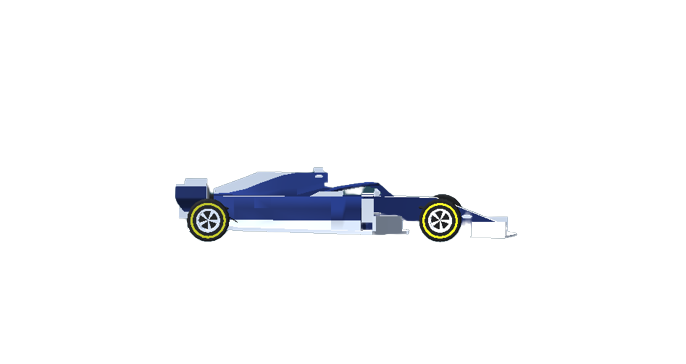
\includegraphics[width=15cm]{f21BG.png}
    \caption{La Formule 1 créée sur \textsl{Blender}}
    \label{fig:F1}
    \centering
\end{figure}

\begin{figure}[h]
    \centering
    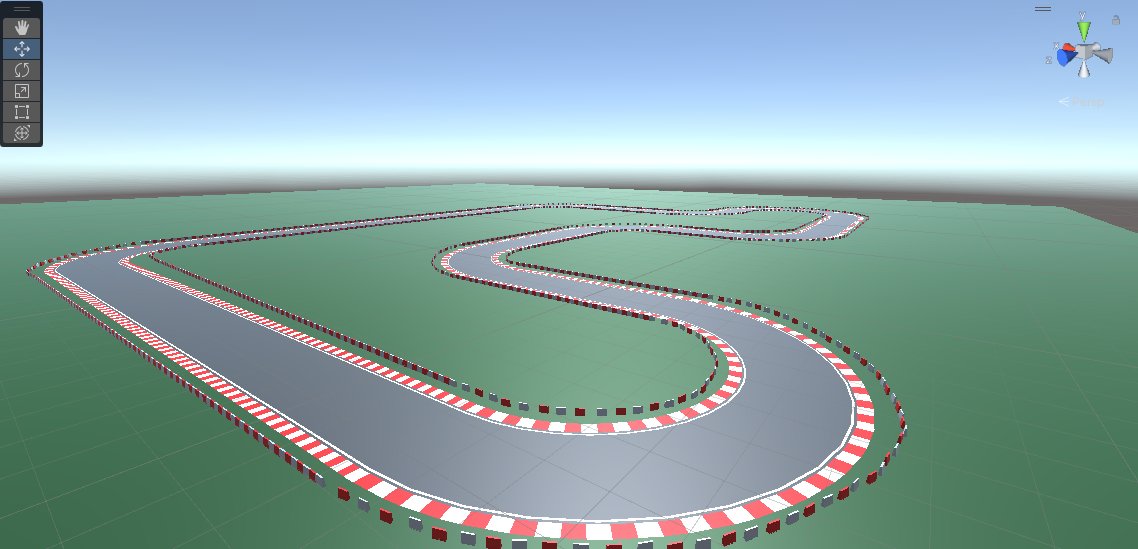
\includegraphics[width=15cm]{circuit.png}
    \caption{Circuit numéro 1}
    \label{fig:track}
\end{figure}

\begin{figure}[h]
    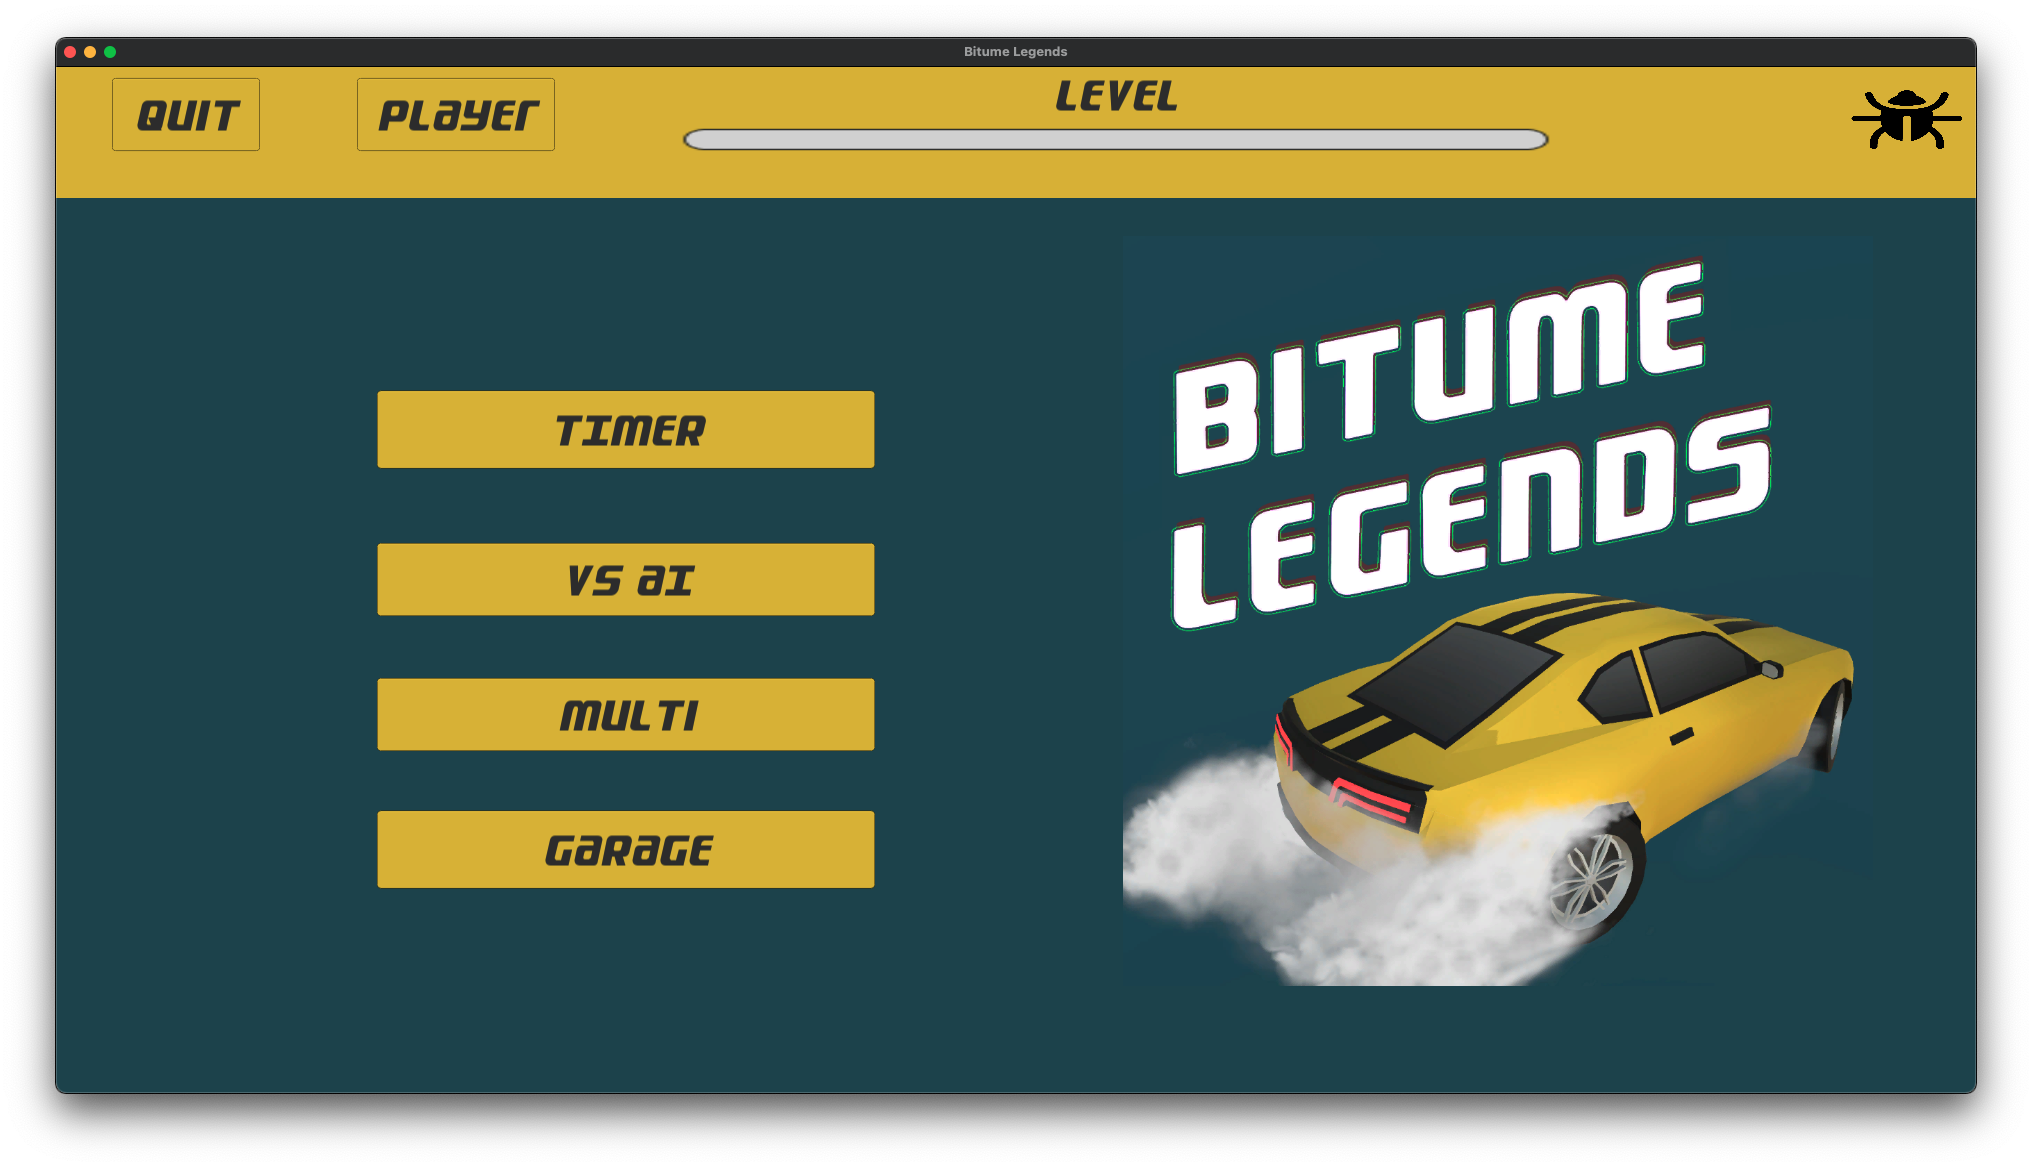
\includegraphics[width=15cm]{menu.png}
    \caption{Le menu principal du jeu}
    \label{fig:menu}
    \centering
\end{figure}

\begin{figure}[h]
    \centering
    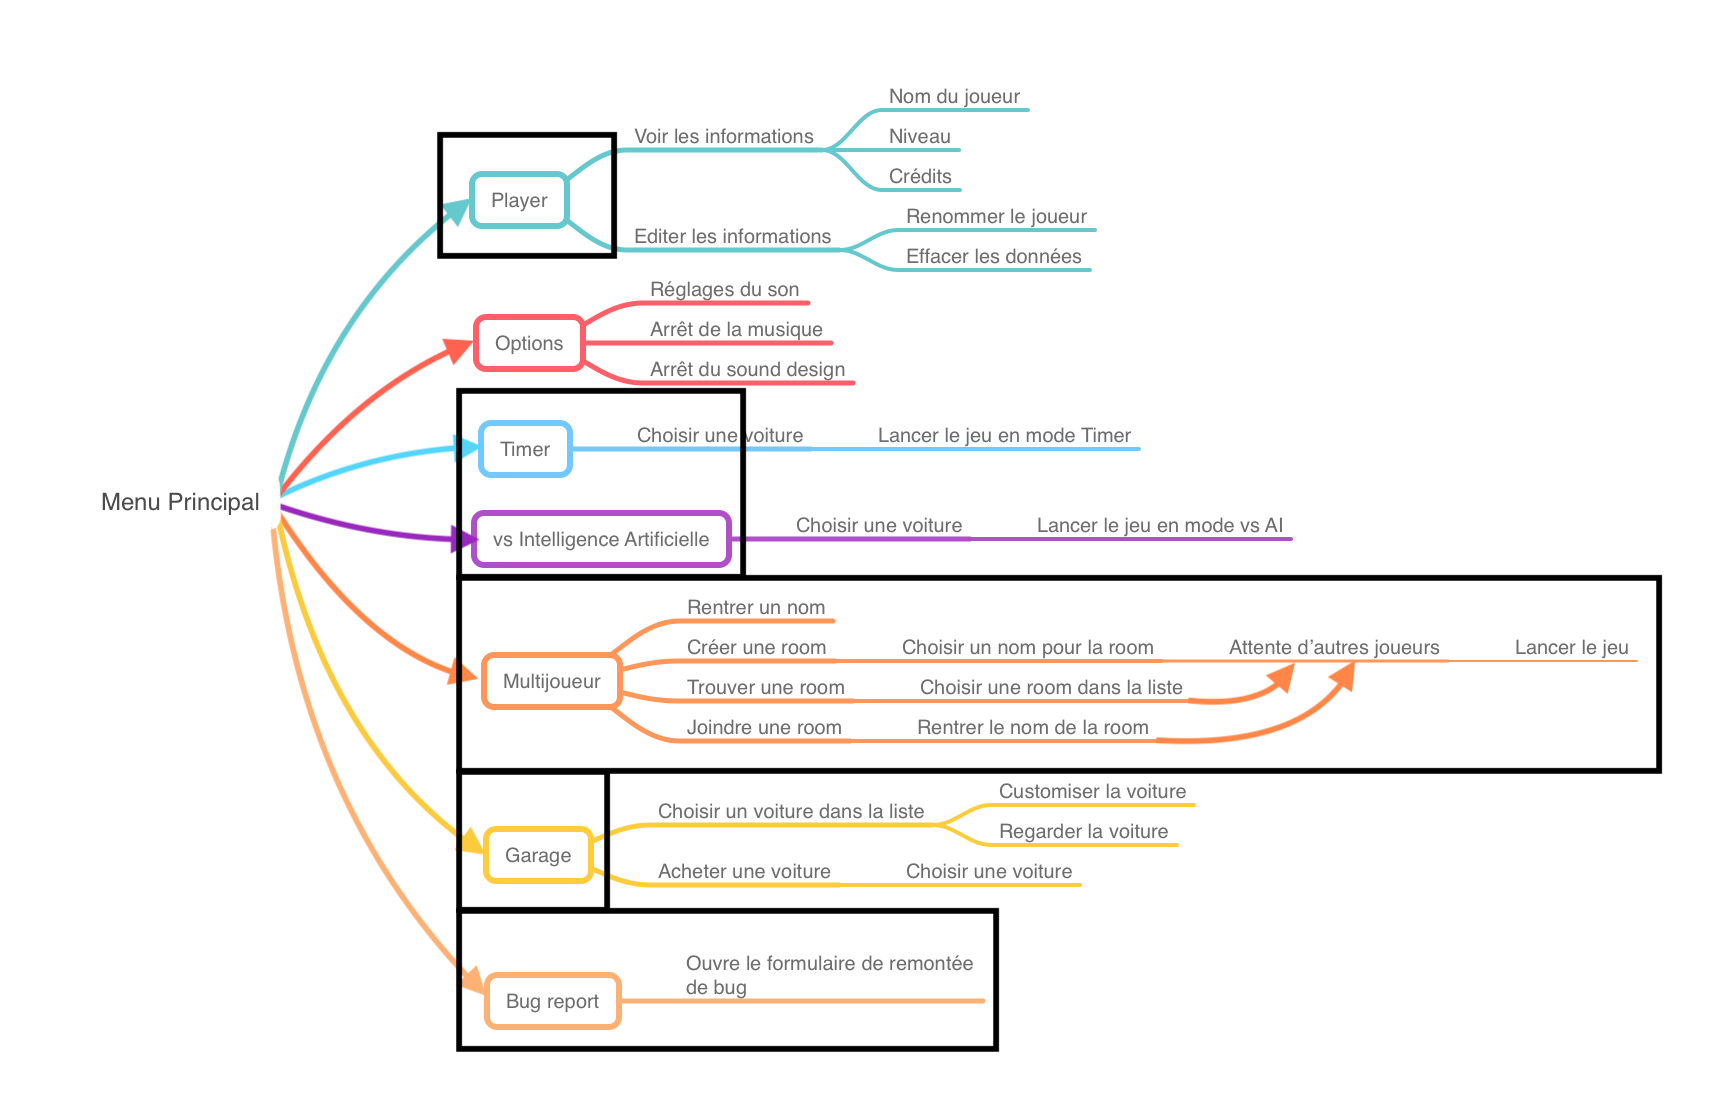
\includegraphics[width=20cm, angle=90]{Menu_Principal.png}
    \caption{Arborescence du menu}
    \label{fig:mindmap}
    Ce qui est entouré est déjà implémenté, le reste suivra.
\end{figure}

\begin{figure}[t]
    \centering
    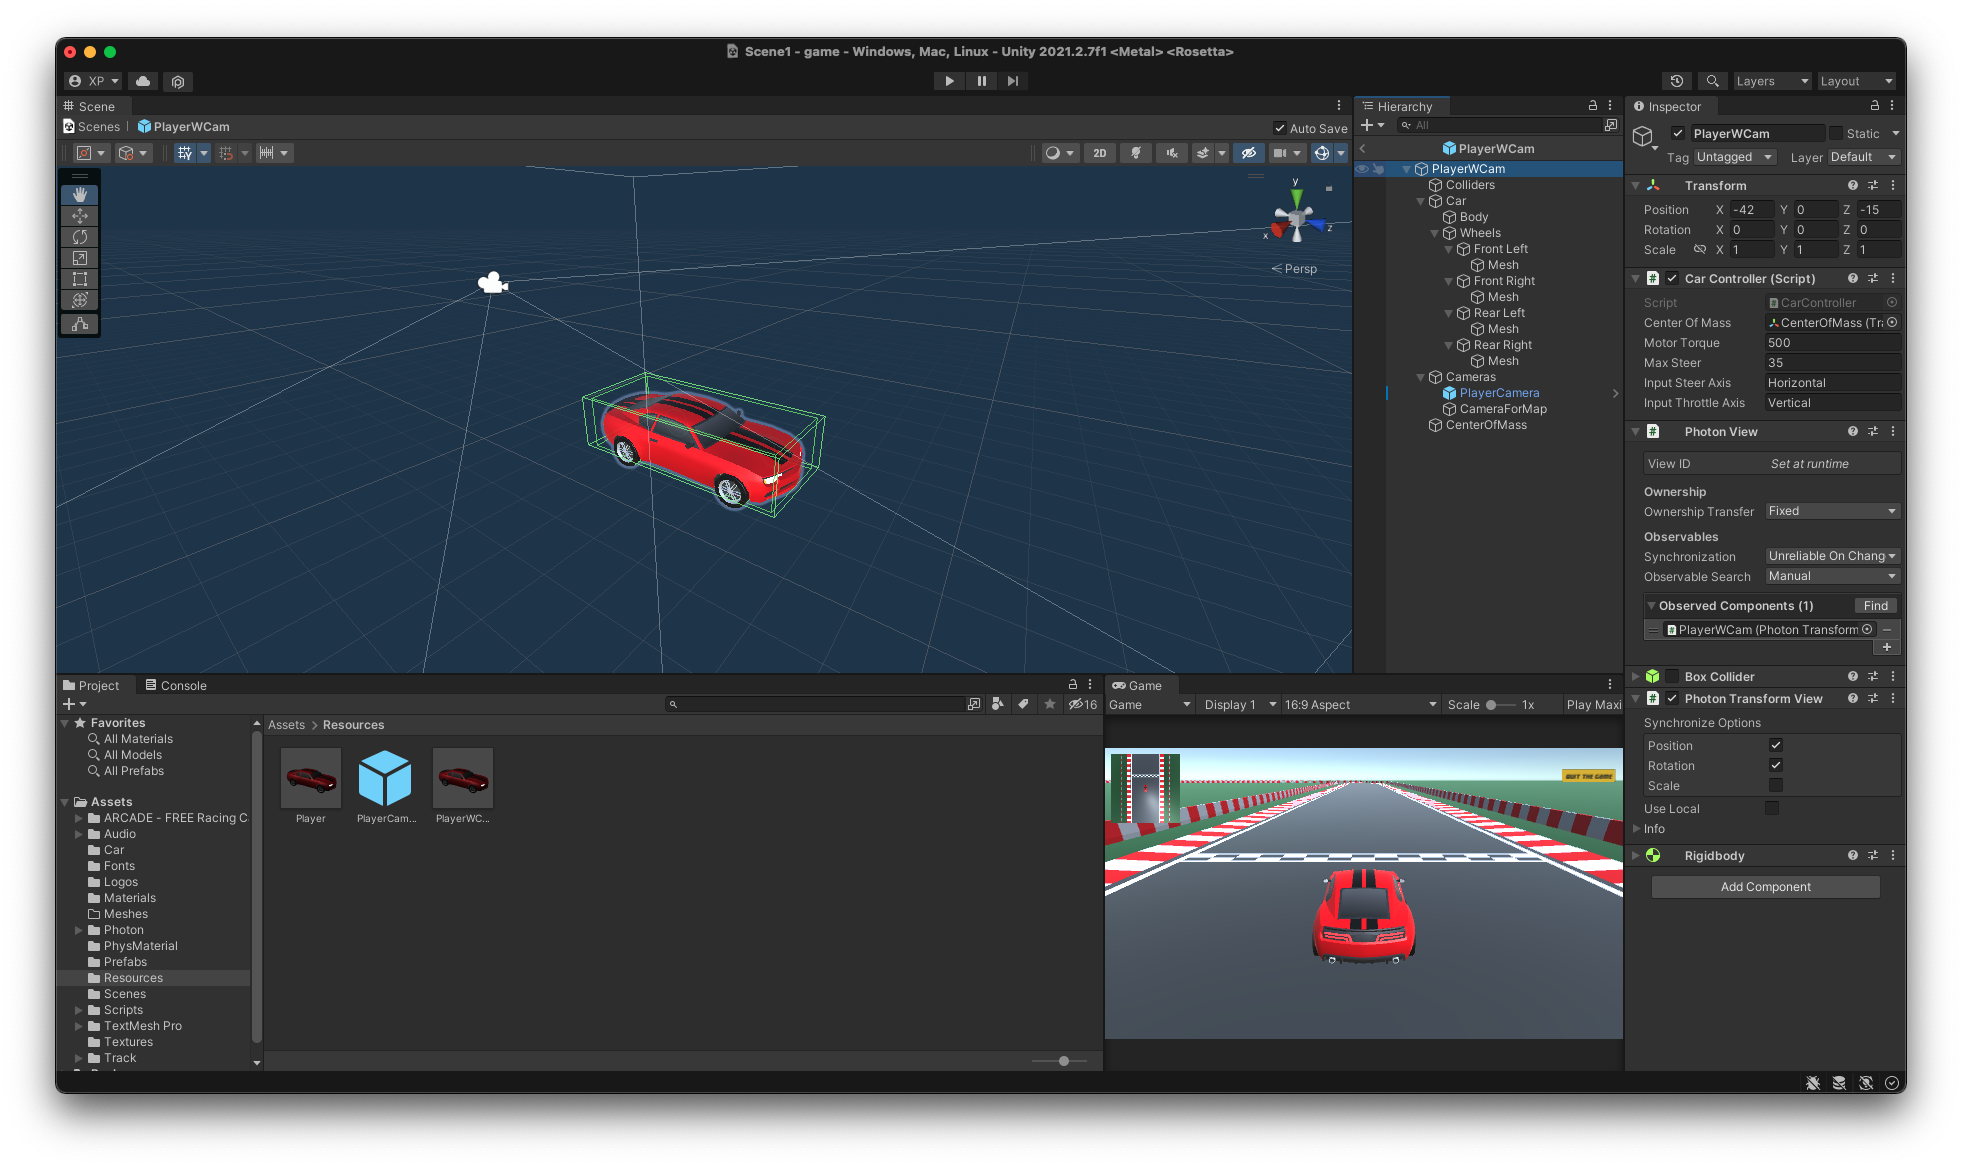
\includegraphics[width=12cm]{prefab.png}
    \caption{Capture de notre voiture équipée}
    \label{fig:prefab}
    Logiciel \textsl{Unity 3D}
\end{figure}

\begin{figure}[h]
    \centering
    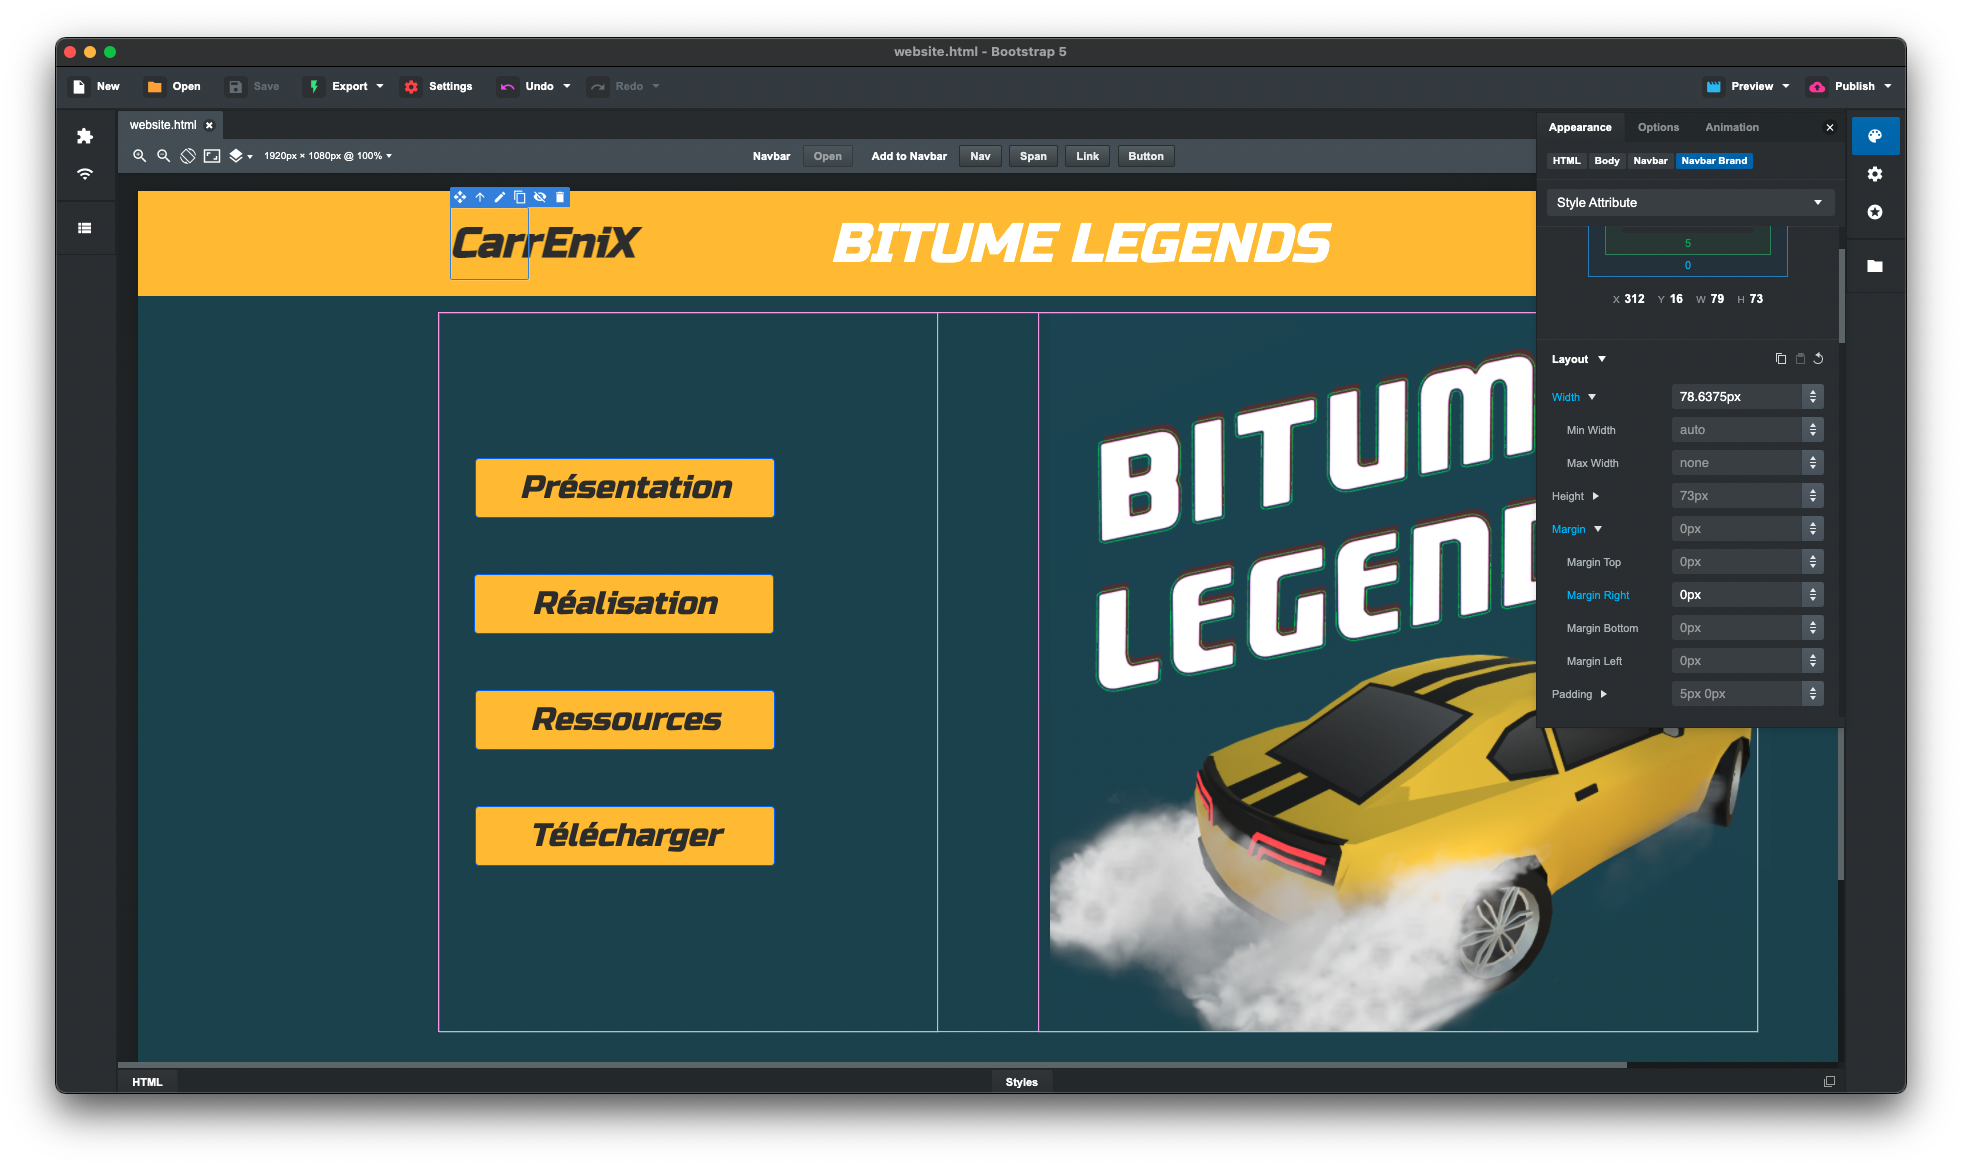
\includegraphics[width=12cm]{bootstrap.png}
    \caption{Capture du logiciel \textsl{Bootstrap Studio}}
    \label{fig:bootstrap}
    (utilisé pour créer le site web)
\end{figure}

\begin{figure}[h]
    \centering
    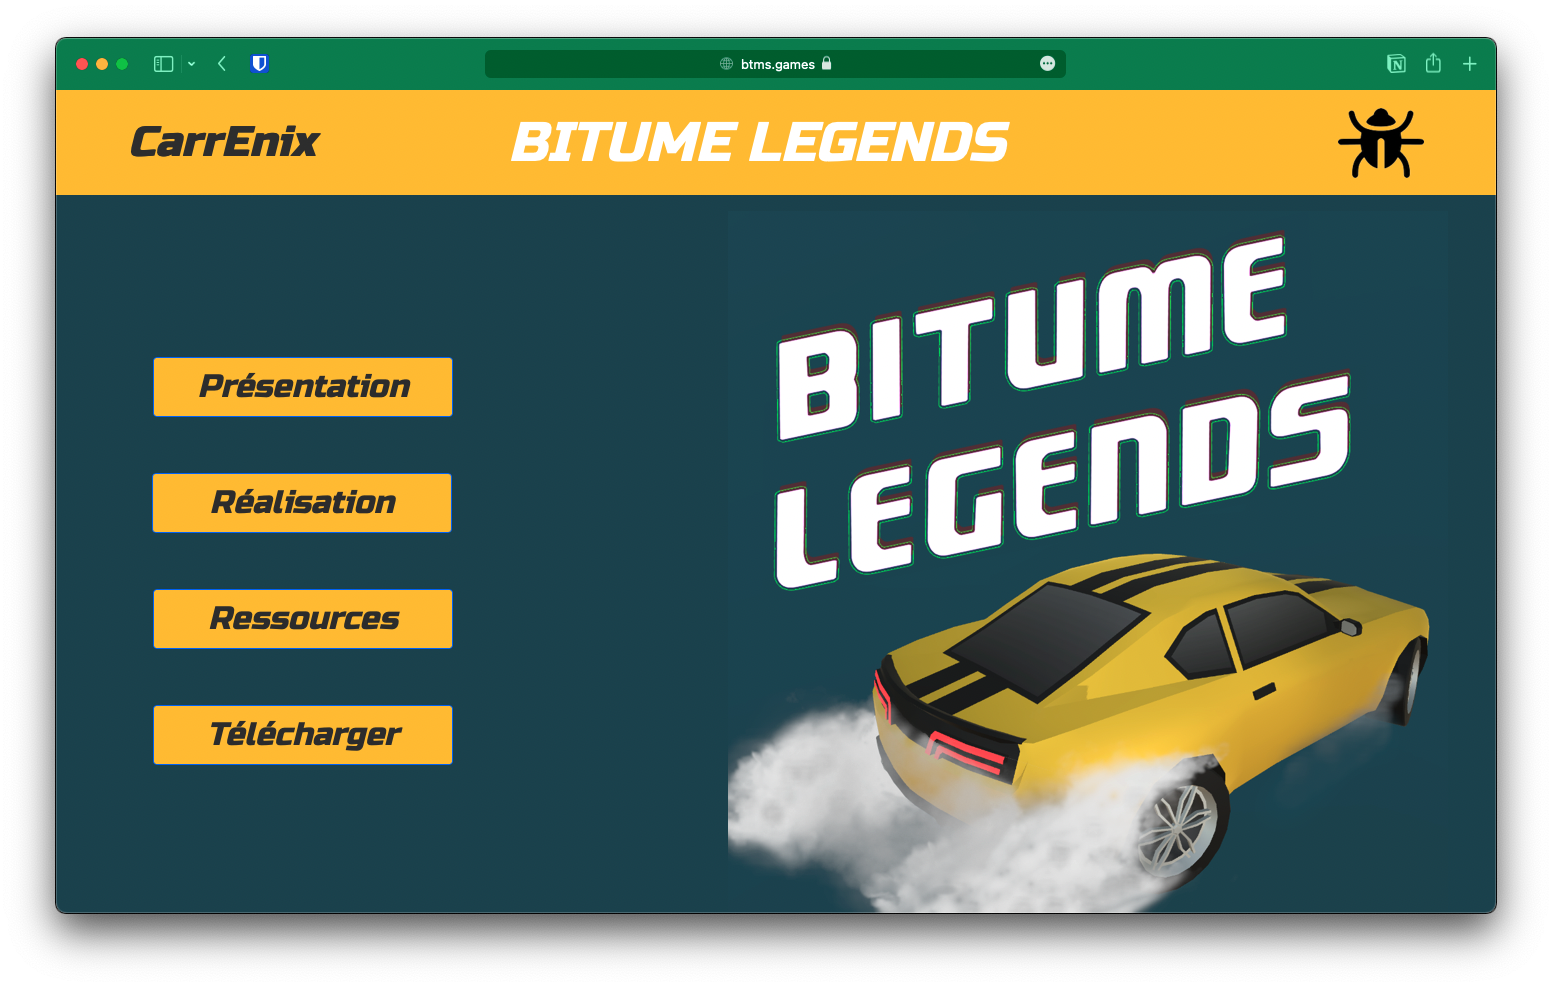
\includegraphics[width=15cm]{site.png}
    \caption{Capture du site Internet}
    \label{fig:site}
    \(\mathtt{btms.games}\)
\end{figure}

\begin{figure}[t]
    \centering
    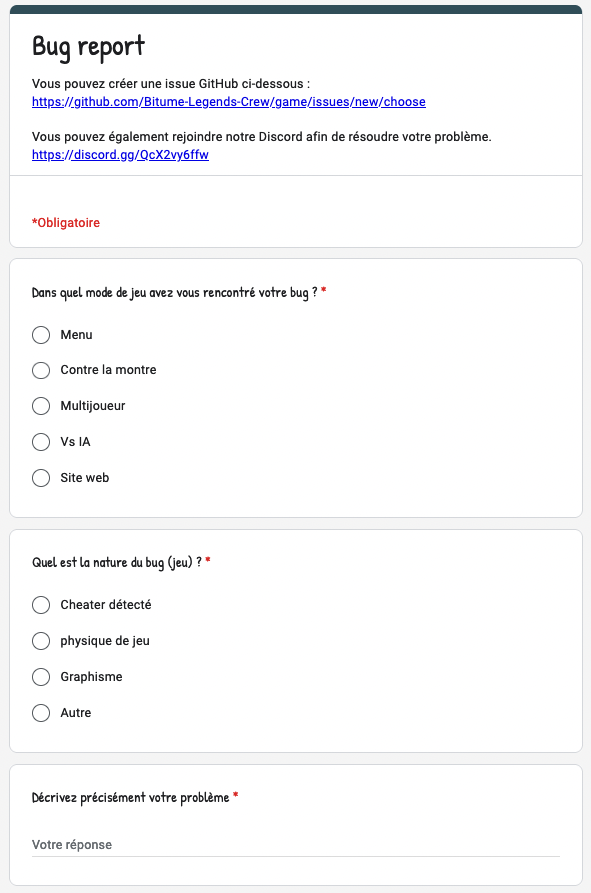
\includegraphics[width=12cm]{bugreport.png}
    \caption{Capture du formulaire de remontée de bugs}
    \label{fig:bug}
\end{figure}

\begin{figure}[t]
    \centering
    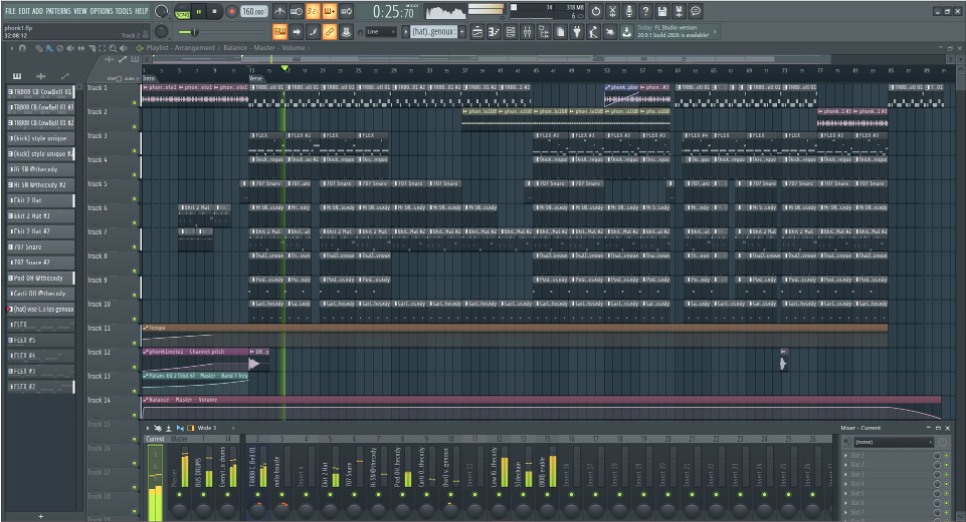
\includegraphics[width=15cm]{zik.png}
    \caption{Capture de la piste de la musique de courses}
    \label{fig:zik}
    \textsl{FL Studio 20}
\end{figure}

\end{document}
